\chapter{Method}
\label{meth}
\label{exp}

Several hypotheses were tested in this work.
Section \ref{data_pp} gives an overview of how input data was pre-processed.
Section \ref{architecture} describes the technical set up required for running all these experiments and deploying the model to production before delving into the specific experiments and their evaluation in section \ref{exp}.

\hfill \break \noindent
The experiments were conducted in five distinct stages:

 \begin{itemize}
   \item Building a visual similarity feature and evaluating its results subjectively.
   \item
    Training a baseline model on the rule-based labels to get a sense of the difficulty of this problem.
    Exploring the predictions subjectively.
   % Since there is no fundamental difference in the way this model was  trained and evaluated compared to the other classifiers, this is described in section \ref{exp_models} with the others. After this step, employees of the client company labeled products that would become the ground truth dataset. The visual comparison feature was also subjectively evaluated at this stage.
   \item
    Training the independent classifiers to determine best performers (\ref{exp_models}).
    Due to the good performance of individual models, ensembling was not attempted due to the engineering overhead it would incur.
   \item Experimenting with different multi-objective learning approaches to determine the most performant way to classify products into exclusive categories.
   \item Training 10 iterations of active learning on the strong predictor (\ref{exp_al}).
 \end{itemize}

There are many kinds of experiments conducted; the experiments, their evaluation and results are explained under the same subsection.
In section \ref{exp_sim} three visual similarity approaches are described and subjectively evaluated;
in section \ref{exp_models} we describe all the models that were trained to reproduce the behaviour of the rule-based system;
how multi-objective learning was used to improve the accuracy of individual training objectives is described in section \ref{multiobj};
finally, our efforts to reduce label complexity using active learning is described in section \ref{exp_al}.


\section{Visual Similarity}
\label{exp_sim}

Three approaches were tried for computing visual similarity.
In the first case, an approximate nearest neighbour method \cite{nmslib} was used on the image embeddings (as described in section \ref{vis_sim_pp}) and the top 100 predictions were saved to ElasticSearch.
In the second approach, the embedding vectors were discretised according to \cite{vec_fulltext} (as described in section \ref{bg_sim}) and inserted to ElasticSearch as strings of space-delimited tokens; standard ElasticSearch fulltext search was used on these token strings to get the nearest neighbour for a given product.
The third approach combined the similarity scores of the second approach and the original ElasticSearch title matching, as a single ElasticSearch query.

\subsection{Evaluation \& Results}

The evaluation of similarity scores is difficult, since it is inherently somewhat subjective.
A common approach is to hand-label triplets of images Q, A, B with four choices: (1) both A and B are similar to query image Q, (2) both A and B are dissimilar to Q, (3) A is more similar to Q than B, and (4) B is more similar to Q than A.
These labeled triplets can be ranked using with similarity precision (percentage of triplets correctly ranked) and score at top K (see \cite{imgsimfineg}).
Creating this dataset of triplets would be a very time-consuming process. Therefore evaluation was done entirely subjectively.

Comparing the similarity between the former ElasticSearch title (ES title) matching and the new approximate nearest neighbour (ANN) search was straightforward - one look at the results was enough to confirm that the embedding-based approach outperforms title matching.
Figures \ref{shirt_es} and \ref{shirt_nmslib} show the nearest neighbours according to ES title and ANN, respectively; the image embeddings nicely pick up the pattern on the shirt, as well as the general style, but also seems to prefer pictures with no fashion model.
For some clothing categories this worked remarkably well, but with categories that had more varied products within it, there were occasional odd results.
For example, in the ``Hiking'' category, the nearest neighbours of sleeping bags could be items with seemingly similar shapes, such as a flashlight that a very zoomed-in product photo that had similar contours as an unrolled sleeping bag.
Another example of this is given in figure \ref{chair_nmslib}, which mostly returns chairs that are indeed visually and even functionally very similar to the chair in question - more so than the ElasticSearch title match seen in \ref{chair_es} - but also returns tables with similar legs; this is understandable, given that nearly half of the surface area of these images is covered by these foldable legs, which are visually quite unique.
This problem can mostly be mitigated by having more fine-grained product categories and restricting the nearest neighbour search to those more specific categories.
The nearest neighbour similarity search may pick up qualities of the image that are not related to the product in question, such as background or fashion model; this is un-intended but is acceptable, and it could be argued creates a product listing which is more homogenous and therefore more aesthetically pleasing.

The second approach of discretised and tokenised image embeddings had mixed results.
The returned nearest neighbours were reasonable, but subjectively felt inferior to the ones computed from the raw image embeddings using ANN.
At times it felt like some aspect of the appearance dominated, which is understandable considering a lot of precision is lost when discretising the embeddings, and there is no theoretical justification why a TF-IDF score of these arbitrarily discretised tokens should behave similarly as a dot product between the original vectors.
With enough precision (using several discrete intervals per embedding dimension) this may well work, but this would incur a considerable performance overhead when indexing and querying.
A hybrid approach was also attempted, where the tokenised version is used to come up with a small set of candidate nearest neighbours, which are used for a precise nearest neighbour calculation; the latter was implemented as an ElasticSearch plugin that performed dot products on the raw embedding vectors, but this was not a scaleable solution and did not subjectively lead to particularly good similarity results.

The third approach of combining the existing title matching and discretised and tokenised vectors was somewhat successful.
As seen in figure \ref{chair_tokenised}, the title matching ensures that top results are at least about the same kind of items (chairs) while the tokenised embedding query returns products that share some visual similarity (mostly the legs of the chair).
This approach still suffered from similar problems as the second approach - poor performance and somewhat inconsistent visual similarity - while introducing an additional complication of finding a good weighting between the title and visual scores.
Given that there was no efficient way to evaluate the different weightings, it was decided to use raw image embeddings for visual similarity, either as an ANN or a precise realtime version.

\begin{figure}
  \centering
  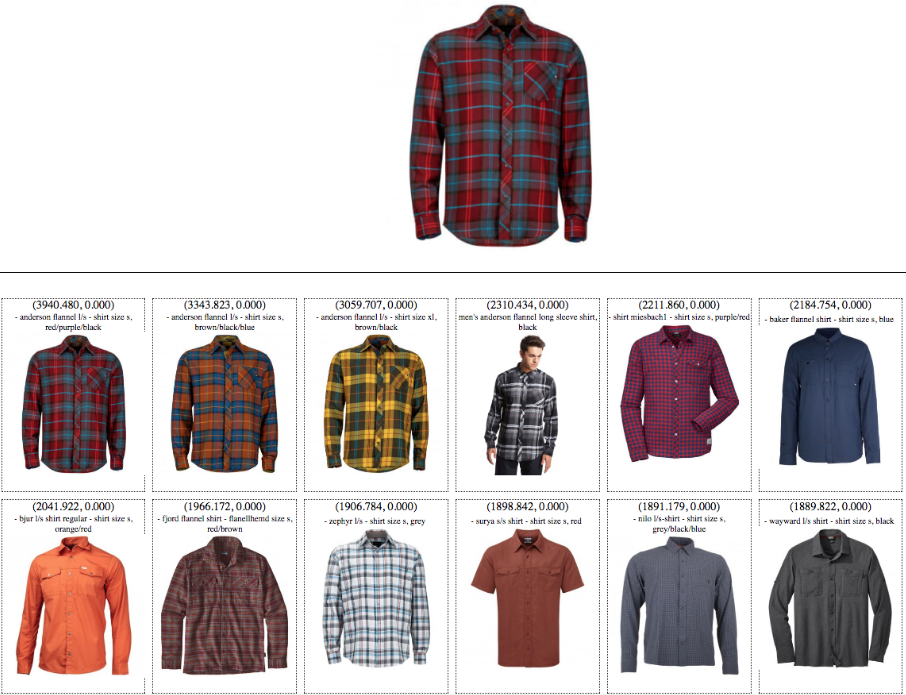
\includegraphics[width=0.8\linewidth]{figures/compare/shirt_es}
  \caption{Nearest neighbours based on ElasticSearch title matching (TF-IDF-like)}
  \label{shirt_es}
\end{figure}
\begin{figure}
  \centering
  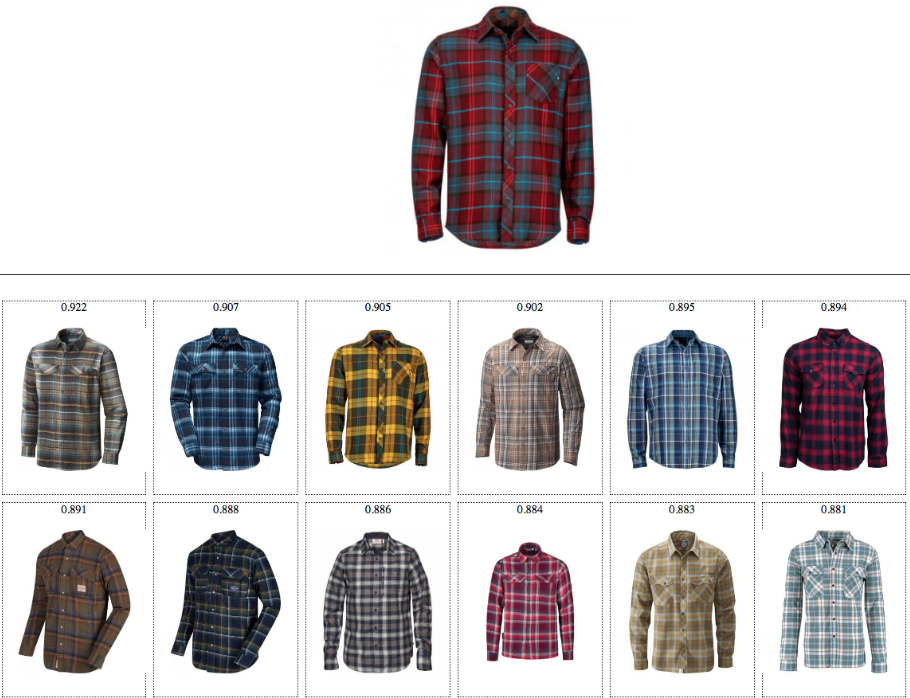
\includegraphics[width=0.8\linewidth]{figures/compare/shirt_nmslib}
  \caption{Nearest neighbours based on ANN search of image embeddings}
  \label{shirt_nmslib}
\end{figure}

\begin{figure}
  \centering
  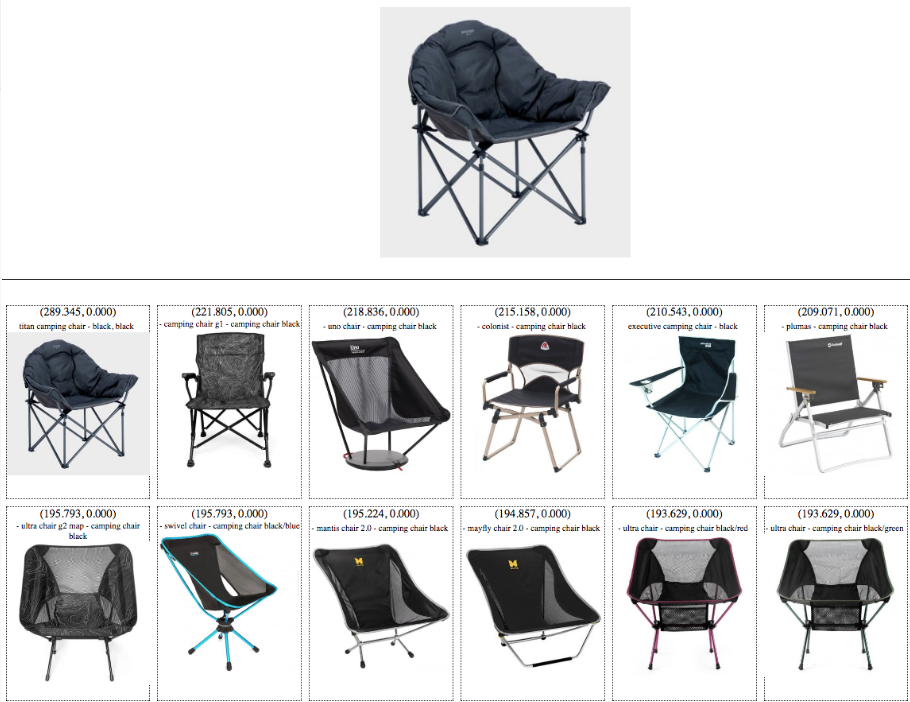
\includegraphics[width=0.8\linewidth]{figures/compare/chair_es}
  \caption{Nearest neighbours based on ElasticSearch title matching (TF-IDF-like)}
  \label{chair_es}
\end{figure}
\begin{figure}
  \centering
  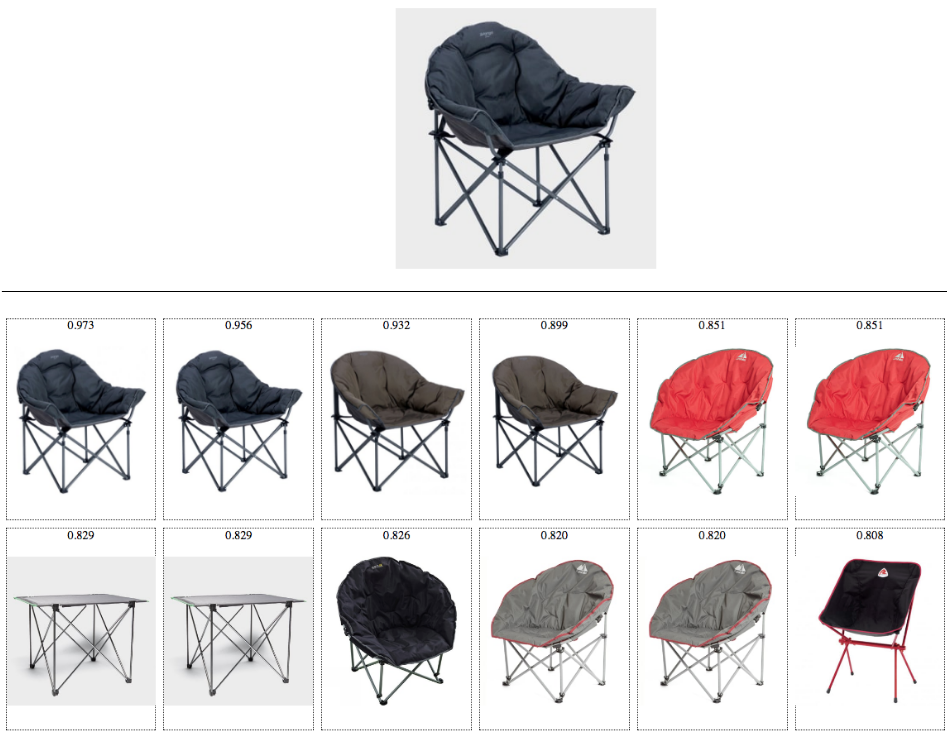
\includegraphics[width=0.8\linewidth]{figures/compare/chair_nmslib}
  \caption{Nearest neighbours based on ANN search of image embeddings}
  \label{chair_nmslib}
\end{figure}
\begin{figure}
  \centering
  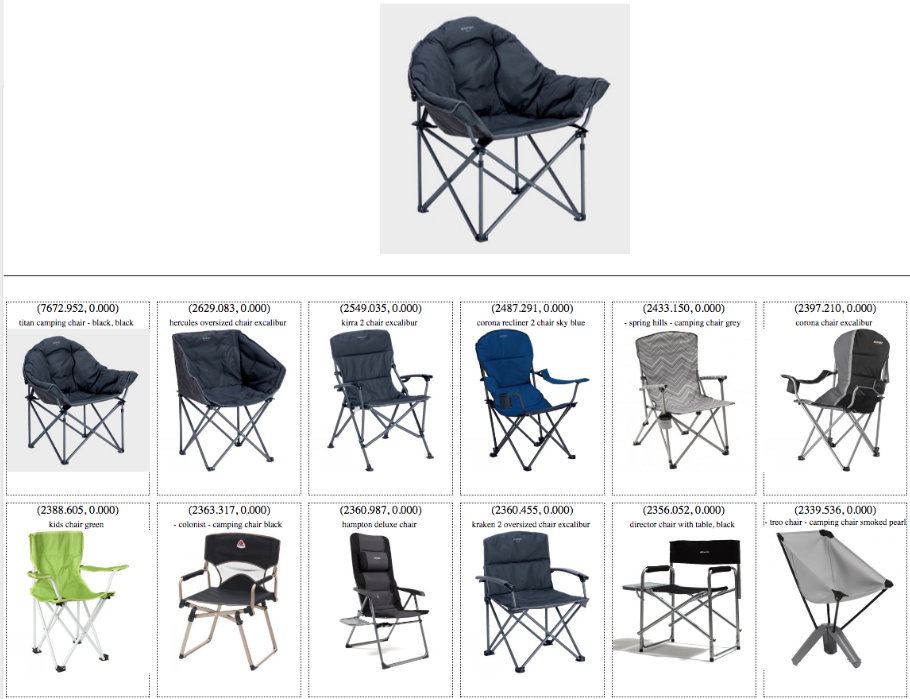
\includegraphics[width=0.8\linewidth]{figures/compare/chair_tokenised}
  \caption{Nearest neighbours based on fulltext search on discretised/tokenised image embeddings as in \cite{vec_fulltext}. Here scores from the title and image embedding fields was combined.}
  \label{chair_tokenised}
\end{figure}

\section{Independent Models}
\label{exp_models}

Several models were trained on the rule-based labels to find out which models can best replicate its behaviour.
We first describe the first model that was trained as a baseline.
Then the different input features and how these were represented are described, along with how linear and deep models were trained from these input representations.
The final section describes how hyperparameters were selected, and two attempts at tuning these programmatically.


\subsection{Evaluation}

Many metrics can be used to evaluate \textbf{multi-label classification}:

\begin{itemize}
  \item TP, TN, FP, FN: true positives, true negatives, false positives, false negatives,
  \item accuracy: $\frac{TP + TN}{FP + FN}$, fraction of correct predictions,
  \item precision: $\frac{TP}{TP + FP}$, fraction of positive predictions that were correct,
  \item recall: $\frac{TP}{TP + FN}$, fraction of positive labels that were correctly ``recalled'',
  \item F1: $2\frac{precision * recall}{precision + recall}$, harmonic average of precision and recall,
  \item TPR = recall: $\frac{TP}{TP+FN}$, true positive rate, probability of detection,
  \item FPR: $\frac{FP}{FP+FN}$, false positive rate, probability of false alarm,
  \item ROC AUC: the area under the curve of TPR plotted against FPR.
  \item PR AUC: the area under the curve of precision plotted against recall.
\end{itemize}

In our case, an overwhelming number of labels are negative, therefore a very simple predictor (that predict ``negative'' for every product / category) would have an accuracy near 99\%; ROC AUC is not suitable for the same reason, as there would be no false positives.
Precision and recall are useful measures to understand the model: it is expected to see a sharp increase of precision and decrease of recall as the model learns to predict ``negative'' for most classes, followed by a gradual increase of recall as the model learns to predict ``positive'' for the correct classes.
Precision and recall are competing metrics: increased precision tends to lead to decreased recall and vice versa, therefore models which combine the two are suitable for evaluating multi-label prediction problems with unbalanced classes.
While F1 score gives the harmonic mean of precision and recall at a given threshold, PR AUC paints a more complete picture by showing what the ratio would be at all the threshold values\footnote{There are infinitely many threshold values in the range 0 ... 1, so naturally we consider a small number of threshold values when approximating AUC.}.
Therefore, all evaluation of multi-label classification is based on PR AUC, i.e. when choosing between model architectures or hyperparameters, a model with a higher PR AUC is preferred.

For \textbf{multi-class classification}, accuracy is still a reasonable measure.
Even though classes are imbalanced (``Dresses'' has more products than ``Travel Books''), there is no single dominant class that could be used as a shortcut by the model.
On the other hand, similar problems arise with evaluating multi-class problems where there is potentially overlap between some classes: the metric would give a low score even if the model predicted a semantically very similar class, or a more general class instead of the more specific one it was labelled as.
Therefore a manual evaluation of the misclassified products is needed to determine whether the error rate is caused by the ambiguity of the classes or by problems with learning.

\subsection{Baseline Model: Wide \& Deep}
\label{widedeep}

As described in section \ref{bg_wide_deep} ``Wide \& Deep'' consists of two models that are trained jointly using stochastic gradient descent: a deep and a shallow neural network which both predict the same set of binary outputs.
The original idea of Wide \& Deep was to use the wide component for feature crosses (e.g. of two categorical values), but in our experiments the wide component received mostly just the 1-hot encoded categorical inputs while the wide component received the same inputs as random embeddings (or as pre-computed image embeddings extracted with Inception V3 that is pre-trained on ImageNet).

Initial experiments with this model were done on a dataset of roughly 800 000 products which were labeled by the rule-based system\footnote{The database in the client company was in constant flux, so the training set sizes depended on how many labels the rule based-system had assigned to the current database}.
The data was partitioned into a train (\textasciitilde80\%), validation (\textasciitilde10\%) and test (\textasciitilde10\%) sets in the Dataflow preprocessing pipeline based on a pseudorandom number generator - assign the product in question to the dataset if the random number is in the range 0 ... 0.8, 0.8 ... 0.9, 0.9 ... 1.
This allowed us to use parallel data preprocessing where workers do not need to be aware of the index of the data point it is processing or what the other workers are doing; due to the randomness the dataset split boundaries will not be exact (e.g. test and validation sets may end up with 12\% and 8\% of products), but this is acceptable given the relatively large dataset size.
The train set was used to train the model, and the validation set was used to evaluate the model periodically as it was trained - during individual training runs and during hyperparameter tuning.
The test set was held out for evaluating the model after hyperparameter tuning, but was not used in this case.

\paragraph{Results}
The PR AUC on the 800,000-item dataset for this model after hyperparameter tuning was 0.9981 (see section \ref{tuning} for a full description of the set-up).
A manual examination of the predictions revealed that the top predictions for most categories was high-quality, but there was a large number of products below the decision boundary that actually belonged above it.
A later run of the model on 1.2M products gave an PR AUC of 0.8647; this was using the hyperparameters that the tuning step produced, so it is likely that the decreased AUC PR score is caused by a bug\footnote{Three possible explanations come to mind: (1) the initial PR AUC was artificially high as some of the test set products ended up in the training set; (2) when migrating from the 800k dataset to the 1.2M dataset, the image embeddings were transferred over as an attempted optimisation approach, which may have mixed up image embeddings between products; (3) the model was overfitting, 10 epochs of 1.2M is effectively 15 epochs of 800k products (the fact that there were more products does not necessarily matter, because labels were assigned simplistically from keyword matches on the title).}.
There were occasional odd results from the model once it was trained on the 1.2M dataset; it was hard to tell which part of the model was causing it, or even whether all the input features are actually improving predictive power; therefore, a more systematic approach was tried, explained in the next section.

\subsection{Input Representation \& Model Type Combinations}
\label{model_comb}

To assess which features are most useful for learning the rule-based objective, different features were grouped into \textit{input types}, shown in table \ref{input_types}.
The columns represent the input feature; refer to \ref{data_pp} for the full feature names and their description.
The entries in the table show how each input feature was represented: \textit{emb} for for categorical features that are represented as random embedding vectors (which are updated during SGD), \textit{emb avg} for multi-token fields where tokens are represented as random embeddings and the input feature is a weighted sum of these embeddings\footnote{Each embedding vector is weighted by the number of times it appears in the input feature, and divided by the L2 norm of the token counts; this gives good results for bag-of-words inputs according to TensorFlow documentation:
\newline
https://www.tensorflow.org/api\_docs/python/tf/feature\_column/embedding\_column}.
Feature columns marked with \textit{u.s.enc} have been converted from raw text into dense embedding vectors of size 512 using a pre-trained model Universal Sentence Encoder \cite{uni_sent_enc}; cells marked with \textit{mobilenet} and \textit{inceptionv3} have respectively extracted image embeddings of size 1280 and 2048 using the Mobilenet \cite{mobilenet} and InceptionV3 \cite{inceptionv3} models that were pre-trained on the ImageNet challenge; these embedding models were used via TensorFlow Hub\footnote{TensorFlow Hub is a collection of TensorFlow models that are pre-trained on some other task and can be used as a feature extractor or as an initialisation for a model that is fine-tuned: https://www.tensorflow.org/hub/}.
Pre-trained models were used only as feature extractors, i.e. were not fine-tuned on our data.

\begin{figure}
  \centering
  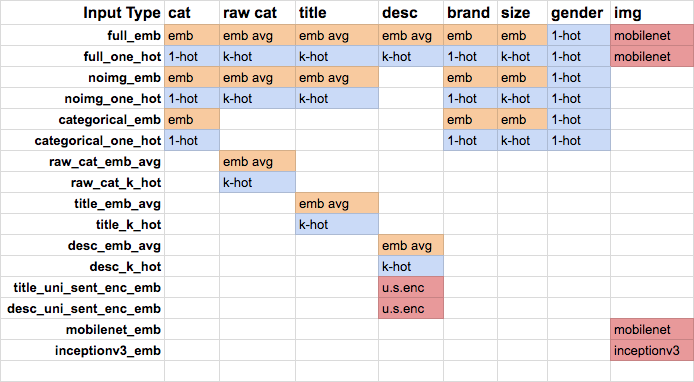
\includegraphics[width=\linewidth]{figures/input_types}
  \caption{Input types. Orange: embedding representation, blue: 1-hot or k-hot, red: embedding extracted with a pretrained deep network.}
  \label{input_types}
\end{figure}

Two model types were used to train with each of these 16 input types: linear and deep.
Like in the case of the baseline model, the \textasciitilde1.2 million data points were split into train/validation/test sets (80\%/10\%/10\%); train and validation sets were used during individual training runs and hyperparameter tuning.
All 32 combinations of input and model type were trained using hyperparameters listed in table \ref{tuning_rounds} column \textit{Deep (rb all)}.

Table \ref{metrics_all} shows the precise PR AUC and recall scores of the final time steps.
The training loss function of linear and deep versions of noimg\_emb is shown in figure \ref{train_loss_all}.
The PR AUC on the validation set is shown in figure \ref{pr_auc_all}, where each model is trained for 300 000 batches, which is roughly 6 epochs; similarly, figure \ref{recall_all} shows how recall changes during the course of training.
The PR AUC on the final step (300k, or 220k for inceptionv3) is shown in figure \ref{pr_auc_chart}; recall plot of the final time step was omitted, as it was very similar to the final PR AUC scores.

\begin{figure}
  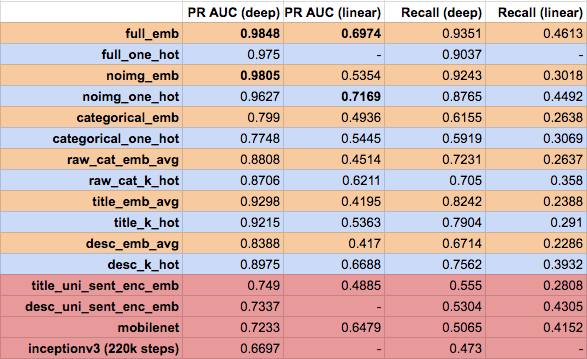
\includegraphics[width=\linewidth]{figures/metrics_all}
  \caption{Evaluation metrics of the rule-based training objective on the final time step. Minus denotes a train run that was not scheduled (inadvertently).}
  \label{metrics_all}
\end{figure}

\begin{figure}
  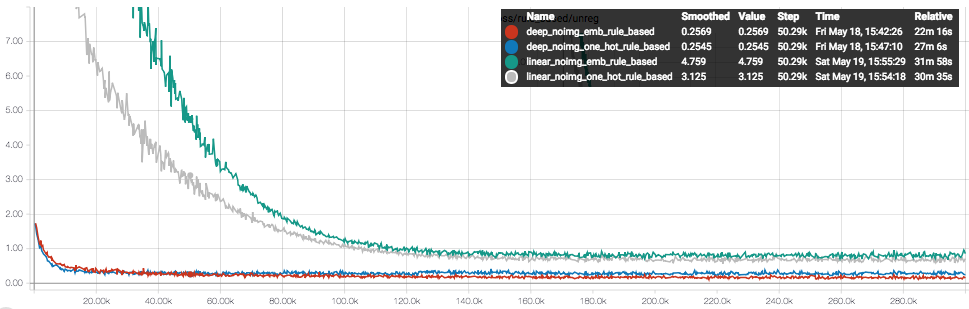
\includegraphics[width=\linewidth]{figures/train_loss_all}
  \caption{x axis = train step (batch number), y axis = training loss of rule-based objective.}
  \label{train_loss_all}
\end{figure}

\begin{figure}
  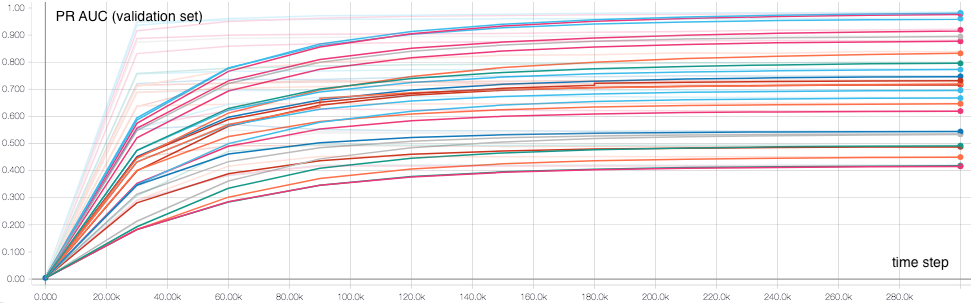
\includegraphics[width=\linewidth]{figures/pr_auc_all}
  \caption{PR AUC of all combinations of input and model types; x axis = train step (batch number), y axis = PR AUC. Refer to figure ... for exact scores.}
  \label{pr_auc_all}
\end{figure}
\begin{figure}
  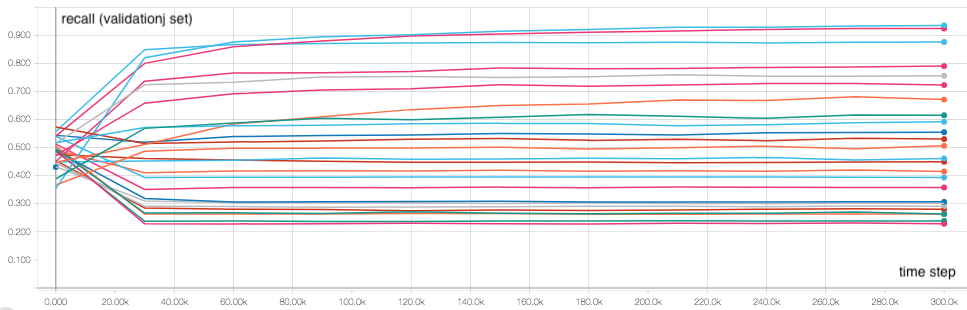
\includegraphics[width=\linewidth]{figures/recall_all}
  \caption{Recall of all combinations of input and model types; x axis = train step (batch number), y axis = recall..}
  \label{recall_all}
\end{figure}

\begin{figure}
  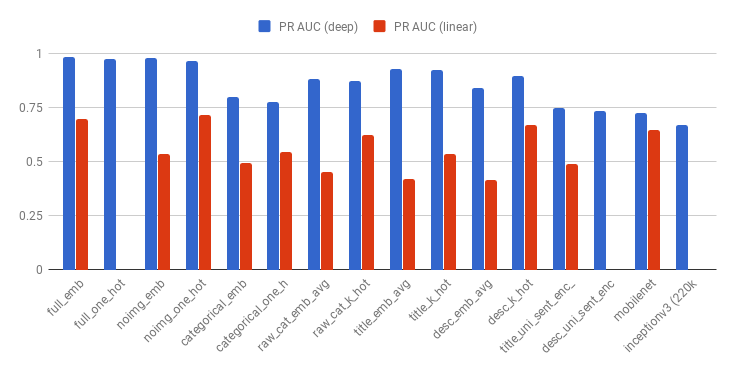
\includegraphics[width=\linewidth]{figures/pr_auc_chart}
  \caption{PR AUC on final timestep (300k, or 220k for inceptionv3)}
  \label{pr_auc_chart}
\end{figure}

\section{Labelling of Exclusive Products}
\label{labex}

There were three purposes for labelling products: (1) creating a validation set, (2) creating an initial dataset for training the exclusive outputs so that reasonable uncertainty scores could be computed for active learning, and (3) labelling during active labelling rounds.
There are three ways of picking products to be labelled: random sampling (a product is sampled randomly from all products that do not have an exclusive label), uncertainty sampling (the unlabelled product with the highest uncertainty score is chosen), and searching for a product manually using our web UI.
Each label that gets persisted has the following metadata associated with it: the label type (\textit{random}, \textit{uncertainty} or \textit{searchFor}), created and modified at timestamps, and ``round''.
Round is used to differentiate between labels from the initial labelling and the active labelling rounds; round 0 corresponds to the validation set, round 1 corresponds to the purpose (2) above, and rounds 2 ... n correspond to active labelling rounds.

In the experiments of the following section, the validation set contained 509 randomly sampled products and 5439 products that were manually searched for; for training set the equivalent numbers were 509 and 5646.
Initially random sampling was used to obtain labels for products, to avoid bias in gathering data only through title search.
Yet this approach would have taken a long time to populate all categories in the validation set with products, therefore the labelling team went through each existing category one by one and added ~5 products to the test and validation set using title matching.

\section{Category Structure}
\label{cat_tree}

At the time of writing, there were roughly 1300 categories defined in the client database.
Categories were structured in a way that is typical of  e-commerce:  categories can have  child categories, which in turn can have child categories, etc.
In our case, the typical depth of the tree structure was five, i.e. a leaf category often had four parents;  naturally, the tree structure was not balanced, so many branches ended at depth three or four.

Categories can be considered as independent (multi-label, sigmoid activation) or mutually exclusive (multi-class, softmax output layer).
The common way to handle this is to assume categories are mutually exclusive.
With exclusive categories, assigning a label to a product determines its label across all categories, whereas with independent categories a positive label only determines the label across the category in question (and its ancestors in the category tree) - that is roughly a thousand-fold difference in labelling efficiency.
The prediction task is also easier for exclusive classes - rather than needing to predict a probability score above a threshold separately for each class, the model would need to just assign the highest probability to the correct class compared to other classes.
On the other hand, some categories at the client company are inherently ambiguous or even overlapping.
The rule-based labels are also independent, since a product may be labelled to belong to zero or many categories.

Bearing in mind the considerable efficiency gain in labelling, we mark a subset of the categories (1063) as ``exclusive''.
Exclusive categories are usually leaves, but at times a higher-level category was marked as exclusive, denoting the more general case\footnote{e.g. if ``Books'', ``Books > Travel Books'' and ``Books > Cookbooks'' are all marked as exclusive, then the semantics of ``Books'' is actually ``Books that are not about travel or cooking''. This means some categories are not strictly exclusive, but we had to work around the existing category structure.}.
Therefore we have two training objectives: a multi-label prediction of independent categories labelled by the rule-based system, and a multi-class prediction of exclusive categories labelled by the employees of the client company - respectively called the \textbf{rule-based} and \textbf{exclusive} training objectives.

We can not use the rule-based labels directly for training the exclusive objective; even if they share the same set of categories, the logits (the value before the softmax/sigmoid activation) of multi-class and multi-label classification behave differently, so we can not just copy the parameters learned from rule-based objective to the exclusive objective.
We can either do multi-objective training where the neural network has two output layers: one for the exclusive and one for rule-based objective.
Alternatively, we could convert the labels assigned by the rule-based system (which are inherently independent) into exclusive labels; we call this training objective \textbf{``exclusivised''\footnote{This word does not exist in dictionaries, but its meaning should be clear.}}.
This would allow us to train with only a single training objective, where most labels are assigned using the rule-based system and ``exclusivised'', and a small number of labels comes from human labellers; this approach might have benefits as the output layer would receive far more examples compared to the exclusive objective in the multi-objective training scenario.
To do that, we look at all the rule-based labels of a product that are applied to categories marked as exclusive.
If there is only one such label assigned, as would be for most products, the label is already exclusive; if there are more than one such label, we can either insert the product to the training set twice (once for each label), or select a random label.
We chose the latter approach.

% \section{Class and Label Imbalance}
\label{label_imbalance}

The labels provided by the rule-based system are only positive:  some products are labelled to belong to a given category, but many products that ought to belong to a category are not labelled  accordingly -  but their label still appears to be negative.
This (which we call the \textbf{label imbalance} problem) only exacerbates the \textbf{class imbalance} problem (that most products do not belong to most categories).
As a result the model trained on rule-based labels will certainly underestimate the likelihood of any product belonging to any category.

\section{Multi-Objective Training}
\label{multiobj}

As described in section \ref{cat_tree} we have three distinct training objectives: \textit{rule-based}, \textit{exclusive}, and a hybrid \textit{exclusivised}.
The models described in the previous section were trained only on the rule-based objective.
In this section we see how a performant models from the previous section performs when trained on the exclusive objective (from a small number of hand-assigned labels), how jointly training using both the rule-based and exclusive objective improves the accuracy of the exclusive objective, and how it compares to the ``exclusivised'' training objective.

Each of the three datasets is represented by a separate set of tfrecords files; these were produced by Dataflow during the preprocessing stage described in section \ref{pp}.
Each objective had two sets of files that corresponded to the training and validation datasets.
For the rule-based objective, this was done based on random splitting; for the exclusive objective, this was done based on a boolean variable the human labeller could specify (``assign this product I am labelling to the train or validation set'').
The exclusivised validation set had the same products as the exclusive validation set, and the exclusivised train set contained all the ``exclusivised'' rule-based labels as well as all the labels from the exclusive train set; when both an exclusivised and manual exclusive label were available, the latter was used.
The train and test set sizes were as follows: rule-based (1.14M / 142K), exclusive (6K, 6.6K), exclusivised (1.24K, 6.6K).

\subsection{Combining Data From Objectives}

To train jointly for the rule-based and exclusive objectives, the data from the different datasets had to be combined.
In the naive version, data from both datasets is loaded into memory and shuffled, but this would not work when we are also loading images or the dataset size grows.
As a scaleable workaround, we read the file names of each objective into memory (a few hundred to a few thousand in our case), shuffle the file names, and alternate between reading $m$ files from the first objective and $n$ files from the second objective (we used $m = n = 1$); when one dataset runs out of files, wrap around, but if the other objective also runs out of files, terminate producing filenames.
The resulting stream of filenames is read by a tf.data.Dataset, which loops through the produced filenames indefinitely and keeps a shuffle buffer of $b$ elements; within this buffer the data points from the different objectives get mixed up, so each training batch usually gets products from both objectives.
Note that the file shards are of different sizes: how many products end up in each file depends on how many Dataflow workers were used and how work was divided among those workers.
Therefore, to avoid long periods where batches are filled with data points from a single objective, larger shuffle buffer sizes should be used.
It takes time to read data from disk into the shuffle buffer, especially with images, so larger shuffle buffer sizes slow down training, as the buffer needs to be re-filled after every time the model is evaluated.

Another simple option for combining data from different objectives is to dump all data in the same file, and optimise the model's parameters with respect to all the objectives for which your items in the given batch have labels for.
This ensures that data points are seen an equal number of times, but is problematic when the different objectives have vastly different number of labels, as there is no good way to force training on the under-represented objective more heavily.
An additional unforeseen problem occurred with this set-up: due to the way data was pre-processed, the data points from the exclusive objective often ended up in a single file, which resulted in terribly unstable training unless the shuffle buffer was the size of the whole dataset.
This can be seen in figure \ref{pretrain}, where the training loss of the rule-based objective (pink) shoots through the roof once it encounters its first exclusive data point.
In this case it happened a late stage, when the model had trained for nearly 4 epochs' worth of data\footnote{Due to the way the input function that feeds data to the model is restarted every time the model is evaluated, there is no guarantee that all files/data points are accessed the same number of times. So it is possible the chunk with all the exclusive labels comes at a late stage or several times.}, and by that time the adaptive learning rate of Adam has already learned that the weights of the exclusive output layer are never updated, i.e. the next update should have a very strong learning rate.
Now when the model sees all the exclusive labels at once, the gradients are big enough to affect the whole network, which is why the changes are visible even in the loss function of the rule-based objective; many other metrics (such as L2 regularisation loss and gradient norm) also grew sharply at the time step when exclusive and rule-based losses blew up.

\subsection{Pretraining on the Rule-Based Objective}

The initial plan was to pre-train the model on the rule-based objective, and then train jointly on both objectives.
As seen on figure \ref{pretrain}, the training loss of the rule-based objective (blue) makes large periodical jumps, followed by periods of high-variance downwards fluctuation.
The first such jump starts when after the first epoch of pre-training, and following jumps can leave the loss function plateaued on the level it jumped to.
The sharp jumps can be explained by the high learning rate set for the parameters of the exclusive output layer that have received few or no updates, and the subsequent plateau of the loss function could be explained by the fact that the learning rate for the rest of the model has been reduced substantially, and the model (which is shaken up from its position near an optimum) is unable to escape its new sub-optimal ``valley'' of the loss surface.
Contrast this with figure \ref{nopretrain}, where the jointly trained model's loss (red) is gradually converging towards the loss of the single-objective loss (blue).
In figure \ref{pretrain} all the other parameters are the same as in \ref{nopretrain}; the former uses pre-training and the latter does not, and obviously the runs had different outcomes when shuffling data.

\begin{figure}
  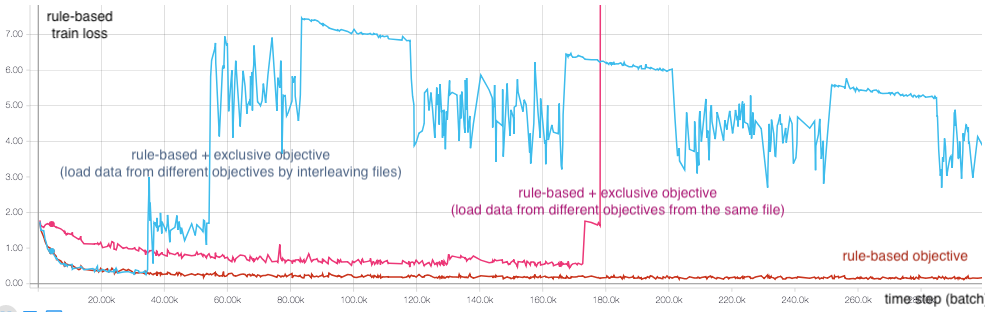
\includegraphics[width=\linewidth]{figures/multiobj/pretrain}
  \caption{Unregularised training loss of rule-based objective. Red: only rule-based objective. Blue: until step 35K, only rule-based objective, then a combination of rule-based and exclusive. Pink: rule-based and exclusive objectives loaded from the same files. Shuffle buffer size: 15K.}
  \label{pretrain}
\end{figure}

\begin{figure}
  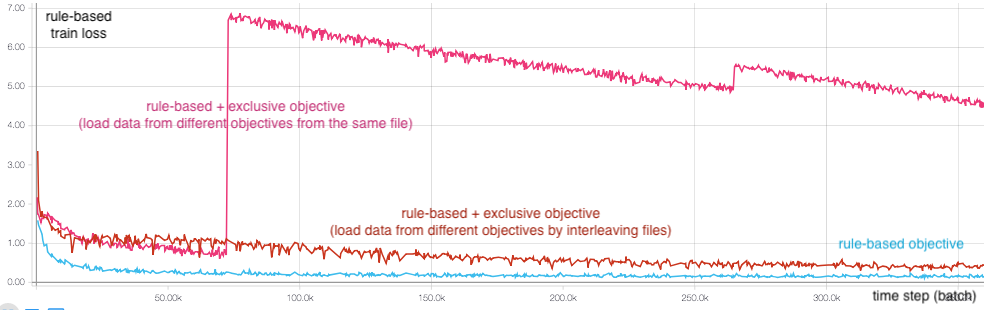
\includegraphics[width=\linewidth]{figures/multiobj/nopretrain}
  \caption{Unregularised training loss of rule-based objective. Blue: only rule-based objective. Red: combination of rule-based and exclusive objective. Pink: rule-based and exclusive objectives loaded from the same files. Shuffle buffer size: 15K.}
  \label{nopretrain}
\end{figure}

\subsection{Exclusive, Exclusive \& Rule-Based, and Exclusivised Objectives}

Our real goal is to properly predict the exclusive objective.
As is evident from figure \ref{ex_vs_joint}, the model trained with just the exclusive objective converges fast and improves little after the first epoch, while the stable multi-objective model continues to improve in accuracy after several epochs, surpassing the single-objective accuracy after about three epochs.
The PR AUC of a model trained on just the rule-based objective exceeds that of the multi-objective training, which can be explained by the additional variance the exclusive objective introduces.
Both results are as expected, though the overall accuracy of 60\% is not particularly strong.
A reasonable guess is that the parameters of the exclusive output layer did not receive enough training examples to learn from, so a model was trained on the exclusivised data set as well.
Alas, as seen in figure \ref{ex_vs_exclusivised}, the exclusivised training objective does not outperform the former multi-objective learning and has a very high variance in the training error; a larger shuffle queue seems to help both settings, however.
As training loss that has a high learning rate would fluctuate similarly when the learning rate is too high, a hyperparameter tuning job was scheduled to find out whether a lower learning rate would provide better results.
Alas, this was not the case, and the poor performance of the exclusivised objective is most likely caused by the noise in the labels.

\begin{figure}
  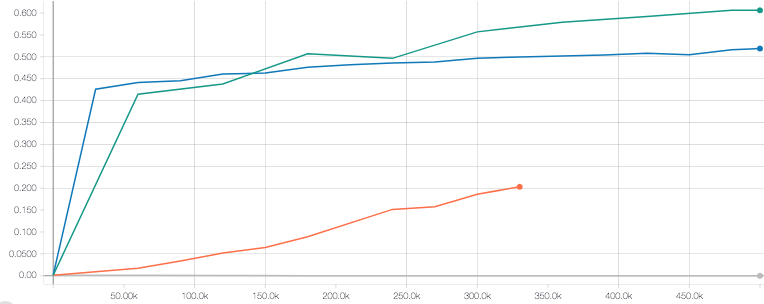
\includegraphics[width=\linewidth]{figures/multiobj/ex_vs_joint}
  \caption{Validation accuracy per time step. Green: multi-objective model (exclusive, rule-based) with interleaved input files. Blue: only exclusive objective. Orange: multi-objective model (exclusive, rule-based) loaded from the same training file (unstable). Shuffle queue: 15K.}
  \label{ex_vs_joint}
\end{figure}
\begin{figure}
  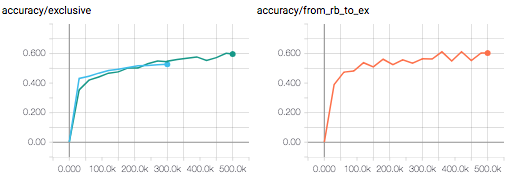
\includegraphics[width=\linewidth]{figures/multiobj/ex_vs_exclusivised}
  \caption{Validation accuracy per time step. Left green: exclusive objective in multi-objective training. Left blue: exclusive objective. Right orange: exclusivised objective. Shuffle queue: 100K.}
  \label{ex_vs_exclusivised}
\end{figure}

To assess whether the low accuracy of 60\% is caused by a genuine problem with learning or an ambiguous validation set, a confusion matrix was computed on the validation set.
Considering there were ~1000 categories, the heat map of the confusion matrix was too dense to reveal useful patterns.
Instead, a histogram of the number of categories that have a given misclassification rate was computed (figure \ref{misclassification_rates}); note that this was computed from both sides of the diagonal of the confusion matrix, therefore a misclassification is counted twice.
Top 20 categories with the highest misclassification rates are shown in figure \ref{misclassified_top}.
The categories with many misclassifications tend to be very general ones; for example, Clothing, Men's Clothing and Casual Shoes are certainly not exclusive, and the client company is advised to find ways of expressing these as exclusive categories.
For some (e.g. ``Knee Length'', ``Mini'', ``Tall''), visual information could be useful which in this round was not used.
The large number of categories that have a single or a handful of misclassifications is most likely caused by a learning problem such as insufficient labels or suboptimal training.

\begin{figure}
\centering
\begin{minipage}{.48\textwidth}
  \centering
  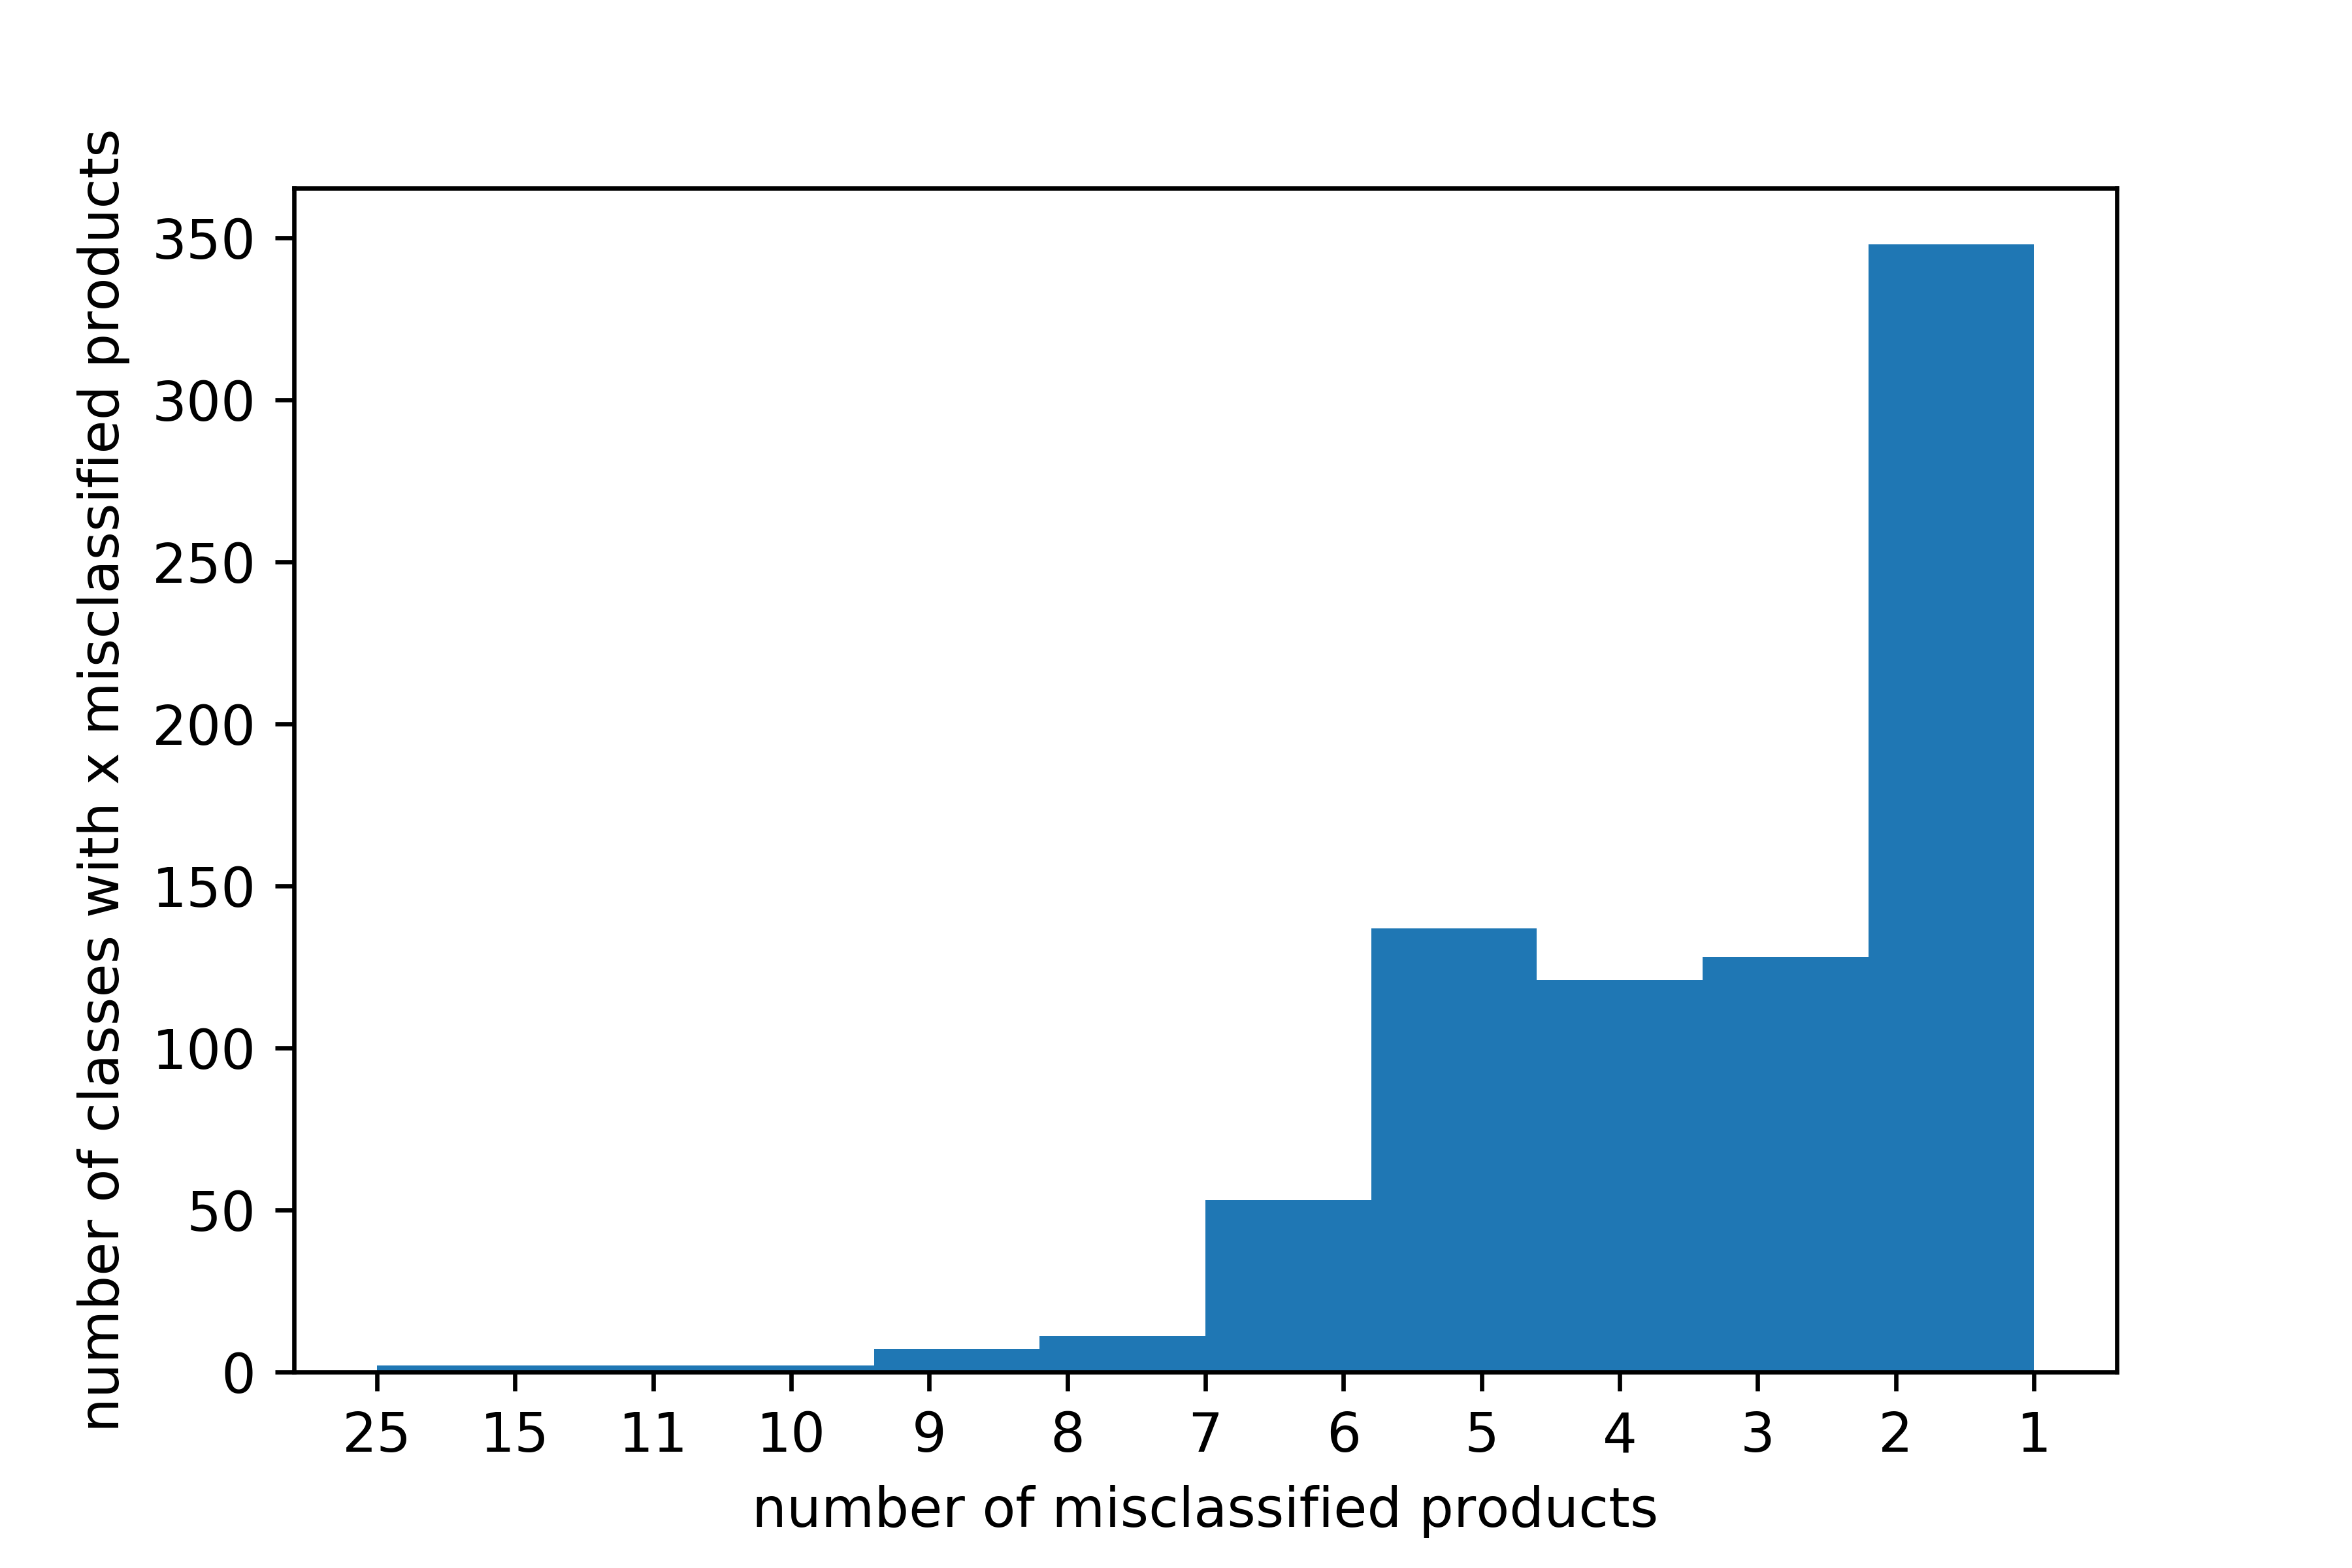
\includegraphics[width=\linewidth]{figures/multiobj/misclassification_rates}
  \caption{Number of misclassified products in validation set.}
  \label{misclassification_rates}
\end{minipage}%
\begin{minipage}{.48\textwidth}
  \centering
  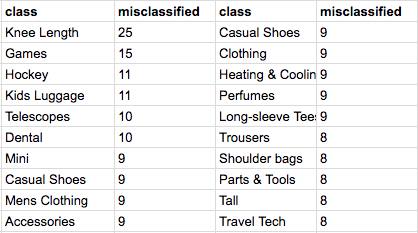
\includegraphics[width=\linewidth]{figures/multiobj/misclassified_top}
  \caption{Worst performers in validation set.}
  \label{misclassified_top}
\end{minipage}
\end{figure}


\section{Hyperparameter Selection \& Tuning}
\label{tuning}

Hyperparameters were chosen based on gut feeling and Bayesian optimisation.
The former was used to come up with reasonable ranges for hyperparameter ranges; automatic tuning was done on the GCP ML Engine, where one just needs to specify the ranges of hyperparameters, their type (categorical, integer, reverse log scale), and how many models are trained in these hyperparameter ranges.
The ML Engine tuning mechanism uses Bayesian optimisation to come up with candidate hyperparameter values, which is described in section \ref{bayesian_opt} and by GCP engineers\footnote{https://cloud.google.com/blog/big-data/2017/08/hyperparameter-tuning-in-cloud-machine-learning-engine-using-bayesian-optimization}.
The hyperparameter ranges used and the results that each of the three tuning rounds found is shown in table \ref{tuning_rounds}.
In all cases 60 models were trained, with maximum 4 models trained in parallel, with early stopping.

The \textit{L2 scale} parameter is the weighting factor on the L2 regularisation term that is applied across the weights of the linear and deep models.
\textit{Linear learning rate} is the learning rate of the Adam optimiser for the linear part of Wide \& Deep, or the weights of the linear model; the other parameters of the optimiser were left as defaults (TensorFlow and the original paper); similarly for \textit{deep learning rate}.
Dropout corresponds to the likelihood of dropping out a hidden unit during training; \textit{layers} corresponds to the number of hidden layers, and \textit{hidden units} corresponds to the number of units in those hidden layers; \textit{activation} corresponds to the activation function used in the hidden layers; the four hyperparameters are only applicable to the deep and Wide \& Deep models.

Table \ref{tuning_rounds} shows the the tuning rounds in different colours, as well as the PR AUC achieved by each.
In the \textit{Wide \& Deep} case, tuning was performed over \textasciitilde800k data points on the rule-based objective, with each model trained up to 6 epochs (e.g. 125k time steps with a batch size of 64).
In the \textit{Deep (rb title)} case, a random sample of 10\% of the full 1.2M dataset was used to train on the rule-based objective for up to 50k time steps; the model used was deep\_title\_emb\_avg, which showed good results compared to the small selection of models that was manually tried.
In the \textit{Deep (exclusivised)} case, the deep\_noimg\_emb model was trained on the full 1.2M dataset on the \textit{from\_rb\_to\_ex} objective (described in section \ref{multiobj}) for up to 300k time steps.
In the {Wide \& Deep} and \textit{Deep (rb title)} cases, models with a higher PR AUC score were preferred while in \textit{Deep (exclusivised)} accuracy was used to choose between hyperparameter performance.

It is clear that the hyperparameters found by the \textit{Deep (exclusivised)} round were not optimal, therefore the ones used in the \textit{Deep (rb all)} was used in most experiments described in section \ref{model_comb}.

\begin{figure}
  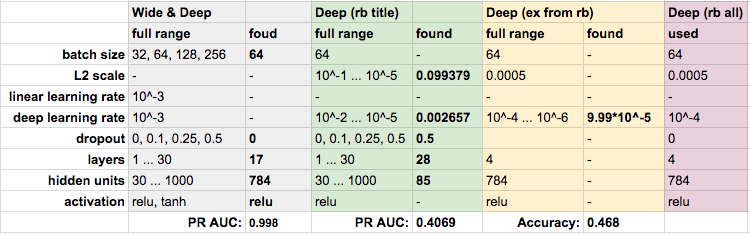
\includegraphics[width=\linewidth]{figures/tuning_rounds}
  \caption{Hyperparameter ranges and the values found during automatic tuning. A single value in the ``full range'' column means the value was fixed.}
  \label{tuning_rounds}
\end{figure}

\section{Active Learning}
\label{exp_al}

Active labelling was used in two ways.
In the first case, the full\_emb model was trained on the rule-based objective, and the entropy of the rule-based prediction was calculated for each product, summed across all classes of the product.
Ideally we would have also tried disagreement sampling, but this would have involved loading predictions from different models across a large number of large files\footnote{To store probabilities for 1000 classes across 4M products as 32bit floats, one needs 16GB; multiply that with the number of models you need to compare uncertainty between.}, which is not only slow but can easily introduce bugs related to misaligned predictions (i.e. products are in a different order across the predictions of different models).
The products returned by this method were in some sense what one might expect - at times returning products that were tricky to label or did not yet have a category - but the products were very similar to one another. Therefore this labelling round was aborted.

The entropy of the rule-based objective was supposed to serve just as a surrogate for the exclusive uncertainty, as the following labelling rounds were supposed to be based on the entropy of the exclusive predictions.
Therefore the labellers were instructed to provide at least 5 labels for each exclusive category (both in the training and validation sets).
Then a deep noimg\_emb model was trained in a multi-objective setting until convergence, and the entropy of the exclusive output is used for sampling products for labelling (deterministically, highest entropy first).

Active labelling would be conducted in rounds as described in section \ref{labex}.
At each round, an equal number of products are labelled using random sampling and uncertainty sampling.
After each round, three models are trained in a multi-objective manner.
The rule-based objective is common to all three, but the number of exclusive labels is different in each: one is limited to randomly sampled labels, one is limited to uncertainty-sampled products, and one uses both.
In all three cases the labels obtained in round 1 using text-based search are included.
In this setting it should be possible to determine whether uncertainty sampling helps us increase validation accuracy faster than random sampling.

The first round of active labelling (round 2 in total) is under way.
Very preliminary results show that uncertainty sampling on the exclusive objective also tends to choose a very narrow range of products to be labelled, though those are such products that it would be expected to be uncertain about, e.g. niche books that do not contain the word ``book'' anywhere in its data, or products for which there is no correct category..
